\documentclass{beamer}

\useoutertheme[glossy]{wuerzburg}
\useinnertheme[shadow,outline]{chamfered}
\usecolortheme{shark}
\beamertemplatenavigationsymbolsempty 

\usefonttheme{professionalfonts}
\let\digamma\relax
\usepackage[scale=0.85,stdmathitalics=true,romanfamily=casual]{lucimatx}
\usefonttheme[stillsansseriftext]{serif}


\usepackage{fancyvrb}

%% Fancy syntax coloring via pygments
\usepackage{minted}
\definecolor{bg}{rgb}{0.95,0.95,0.95}
\usemintedstyle{borland}


\newenvironment{Rcode}
{\VerbatimEnvironment
 \begin{minted}[fontsize=\scriptsize,baselinestretch=1]{r}}%
{\end{minted}}

\newenvironment{Pcode}
{\VerbatimEnvironment
 \begin{minted}[fontsize=\scriptsize,baselinestretch=1]{python}}%
{\end{minted}}

\newenvironment{Code}[1]
{\VerbatimEnvironment
 \begin{minted}[fontsize=\scriptsize,baselinestretch=1]{#1}}%
{\end{minted}}


\usepackage{textfit} % commands \scaletoheight{height}{text} and \scaletowidth{width}{text}

\usepackage{tikz}


\newtheorem{Alert}{Alert}
\newtheorem{Highlight}{Highlight}

\newcommand{\Species}[1]{{\rmfamily \itshape #1}}
\newcommand{\Real}{\ensuremath{\mathbb{R}}}
\newcommand{\RealN}{\ensuremath{\mathbb{R}^n}}
\newcommand{\RealP}{\ensuremath{\mathbb{R}^p}}
\newcommand{\Mtx}[1]{\ensuremath{\mathbf{#1}}}
\newcommand{\Inv}[1]{\ensuremath{#1^{-1}}}
\newcommand{\InvMtx}[1]{\ensuremath{\mathbf{#1}^{-1}}}
\newcommand{\Red}[1]{\textcolor{red}{#1}}
\newcommand{\PsInv}[1]{\ensuremath{\mathbf{#1}^{+}}}



%===========================================================
% Title Info
\title{Scientific Computing for Biologists}
\subtitle{Biology 313\\
Fall 2011\\
Tue 2:50-5:20
}

\author[P. Magwene]{Instructor: Paul M. Magwene}

\institute[Bio 313]{
Email: paul.magwene@duke.edu\\
Phone: 613-8159
}

\date{30 August 2011}

\begin{document}
%===========================================================
\begin{frame}
\titlepage
\end{frame}

%===========================================================
\begin{frame}
  \frametitle{Overview of Lecture}
  
\begin{itemize}
		\item Course Mechanics
		\begin{itemize}
			\item Goals of course
			\item Structure of lectures
			\item Grading
			\item Survey of previous training
		\end{itemize}
		\item Introduction to R and Python
		\begin{itemize}
			\item Advantages of R and Python
			\item R and Python Resources
			\item Important programming concepts
			\item Introduction to data types and data structures in R and Python
			\item Literate programming
		\end{itemize}
		\item Hands-On Session
\end{itemize}

\end{frame}


%===========================================================
\begin{frame}
  \frametitle{Class Structure}
\begin{itemize}
	\item Lectures	
	
		\begin{itemize}
			\item Typically 60-75 minutes
			\item Emphasize the mathematical basis of the methods/approaches from both a geometric and algebraic basis
			\item Discuss algorithms underlying the methods
			\item Highlight available R/Python libraries
		\end{itemize}
		
	\item Hands-on
	
			\begin{itemize}
				\item Walk through some examples
				\item Apply the techniques and concepts to real data
			\end{itemize}
	
\end{itemize}

\end{frame}
%===========================================================

%===========================================================
\begin{frame}
  \frametitle{Syllabus}

\scriptsize

\renewcommand{\arraystretch}{1.1}
\begin{tabular}{rp{3.5in}}
\multicolumn{1}{c}{{\sl Date}} & \multicolumn{1}{c}{{\sl Topic}} \\
August 30 & Introduction; Getting Acquainted with R and Python, Literate Programming \\
September 6 & Data as Vectors and Exploratory Data Analysis; vector operations, dot product, correlation, regression as projection, univariate visualizations\\
September 13 & Linear Algebra Review I; Descriptive statistics as matrix operations, multivariate visualizations \\
September 20 & Linear Algebra Review II; Regression models \\
September 27 & Eigenvectors and Eigenvalues; Principal Components Analysis \\
October 4 & Singular Value Decomposition, Biplots, and Correspondence Analysis\\
October 11 & \multicolumn{1}{c}{{\sc Fall Break}} \\
October 18 & Discriminant analysis and Canonical Variate Analysis\\
November 25 & Analyses based on Similarity/Distance I; Hierarchical and K-means clustering\\
November 1 & Analyses based on Similarity/Distance II; Multidimensional scaling\\
November 8 & Randomization and Monte Carlo Methods; Jackknife, Bootstrap\\
November 15 & Building Bioinformatics Pipelines I; Pipes, redirection, subprocesses \\
November 22 & Building Bioinformatics Pipelines II; Putting the concepts to work \\ 
November 29 & Building Bioinformatics Pipelines III; Polishing the interface and generating publication quality graphics \\ 

\end{tabular}

\normalsize

\end{frame}
%===========================================================



%===========================================================
\begin{frame}
  \frametitle{Texts for Course}

\begin{itemize}

\item Janert, P. K. 2010. Data Analysis with Open Source Tools. O'Reilly, Cambridge.

\item Downey, A.\ B., J.\ Elkner, and C.\ Meyers. How to think like a computer scientist: learning with Python. 
\begin{itemize}
	\item Available at \texttt{http://www.ibiblio.org/obp/thinkCSpy/}
\end{itemize}

\item Wickens, T.\ D. 1995. The geometry of multivariate statistics. Lawrence Earlbaum Associates, New Jersey. 

\end{itemize}

\end{frame}
%===========================================================


%===========================================================
\begin{frame}
  \frametitle{Supplementary Texts}
\begin{itemize}

\item R and Python
\begin{itemize}
    \item Jones, O. et al. 2009. Scientific programming and simulation using R. CRC Press.
	\item Martelli, A. (2006). Python in a nutshell (2nd ed.). O'Reilly. 
\end{itemize}
\item Statistics
\begin{itemize}
	\item Krzanowski, W. J. 2003. Principles of multivariate analysis. Oxford University Press.
	\item Sokal, R. R. and F. J. Rohlf. 1995. Biometry. W. H. Freeman.
\end{itemize}
\item Math
\begin{itemize}
	\item Hamilton, A. G. 1989. Linear algebra: an introduction with concurrent examples. Cambridge University Press.
	
\end{itemize}
\end{itemize}

\end{frame}
%===========================================================

%===========================================================
\begin{frame}
  \frametitle{Grading}
\begin{itemize}
\item Problem sets/programming assignments
\begin{itemize}
	\item 8-10 over the course of the semester
	\item Prepared as `literate programming' documents
\end{itemize}

\end{itemize}

\end{frame}
%===========================================================

%===========================================================
\begin{frame}
  \frametitle{Survey on Previous Background}
\begin{itemize}

\item Programming experience?
\item Mathematical preparation?
\begin{itemize}
	\item Linear algebra
\begin{itemize}
	\item Matrix arithmetic - addition, subtraction, multiplication
	\item Dot product - projection, angle between vectors
	\item Matrix inverse
	\item Determinant, rank, subspace
	\item Eigenvectors/eigenvalues
\end{itemize}
\end{itemize}
\item Statistical preparation?
\begin{itemize}
	\item Previous R/S-plus experience
	\item Class in or self-study of multivariate techniques
\end{itemize}

\end{itemize}

\end{frame}
%===========================================================

%===========================================================
\begin{frame}
  
\begin{center}
\LARGE{Introduction to R and Python}
\end{center}

\end{frame}
%===========================================================

%===========================================================
\begin{frame}
  \frametitle{Advantages of R and Python}
\begin{itemize}

\item Both R and Python can be used in an interactive mode

\begin{itemize}
	\item enter commands/instructions at an interactive prompt for immediate execution
	\item facilitates exploratory analyses 
\end{itemize}

\item Large collection of libraries/packages are available for statistical and numerical analysis and visualization

\item Relatively easy to learn

\end{itemize}

\end{frame}
%===========================================================

%===========================================================
\begin{frame}
  \frametitle{Why Both R and Python?}
\begin{itemize}

\item R is geared toward statistical computing
\begin{itemize}
	\item Great set of built-in facilities for statistically oriented tasks
	\item Somewhat cumbersome syntax for non-statistical tasks
\end{itemize}

\item Python is a general programming language
\begin{itemize}
	\item Clearer syntax
 \item Wider range of modules
		\begin{itemize}
			\item web programming, databases, numerical analysis, etc.
		\end{itemize}
	\item More natural language for simulation
	\item More suitable as a `glue' language
		\begin{itemize}
			\item building bioinformatics pipelines
		\end{itemize}
\end{itemize}

\end{itemize}

\end{frame}
%===========================================================

%===========================================================
\begin{frame}

\begin{center}
\LARGE{R Overview}

\end{center}
\end{frame}
%===========================================================


%===========================================================
\begin{frame}
  \frametitle{What is R?}
\begin{itemize}

\item `A language and environment for statistical computing and graphics'
\item First developed in the mid-90s
\item Derives from the S language
\begin{itemize}
	\item S was developed at Bell Labs in the mid-80s
\end{itemize}

\item Advantages

	\begin{itemize}
	\item Free and open-source
	\item Much of the academic statistical community has adopted it
	\item Active developer and user community
	\item Wealth of built-in and user contributed libraries available for all types of analyses
	\end{itemize}

\item Disadvantages
	\begin{itemize}
		\item GUI not as well developed as commercial statistical packages
			\begin{itemize}
				\item S-Plus; site licensed by Duke - see OIT website
			\end{itemize}
		\item Has higher learning curve than some other simpler statistical software
		\item Command-line can be intimidating
	\end{itemize}

\end{itemize}

\end{frame}
%===========================================================

%===========================================================
\begin{frame}
  \frametitle{R Resources on the Web}
\begin{itemize}

\item Home Page
\begin{itemize}
	\item \texttt{http://www.r-project.org}
\end{itemize}

\item Comprehensive R Archive Network (CRAN)
\begin{itemize}
	\item \texttt{http://cran.r-project.org/mirrors.html}
	\item See especially the `Task Views'
			\begin{itemize}
				\item Statistical and population genetics
				\item Environmental and ecological analysis
				\item Spatial statistics
			\end{itemize}
\end{itemize}

\item Introductions and Tutorials
\begin{itemize}
	\item see \texttt{http://cran.r-project.org/other-docs.html}
\end{itemize}

\end{itemize}
\end{frame}
%===========================================================

%===========================================================
\begin{frame}
  \frametitle{Some R Packages of Interest}

\begin{itemize}
    \item Bioconductor -- software package geared towards analysis of genomic data, especially  microarray data, \url{http://www.bioconductor.org/}
        \item ape -- `Analysis of Phylogenetics and Evolution', \url{http://ape.mpl.ird.fr/}
    \item ade4 -- Analysis of Ecological Data : Exploratory and Euclidean methods in Environmental sciences, \url{http://pbil.univ-lyon1.fr/ADE-4/home.php?lang=eng}
\end{itemize}



\end{frame}
%===========================================================




%===========================================================
\begin{frame}

\begin{center}
\LARGE{Python Overview}

\end{center}
\end{frame}
%===========================================================

%===========================================================
\begin{frame}
  \frametitle{What is Python?}
\begin{itemize}

\item High-level scripting/programming language
\begin{itemize}
	\item simple syntax, easy to learn
\end{itemize}

\item Supports a variety of programming paradigms
	\begin{itemize}
		\item Procedural, object-oriented, some functional programming idioms
	\end{itemize}

\item Invented by a computer scientist named Guido van Rossum at the Dutch National Research Institute for Mathematics and Computer Science

\item First publicly released in 1991

\item Named after Monty Python's Flying Circus!
\end{itemize}

\end{frame}
%===========================================================


%===========================================================
\begin{frame}
  \frametitle{Advantages of Python}
\begin{itemize}

\item Active development
\begin{itemize}
	\item stable core
	\item new language features being added
\end{itemize}


\item Extensive standard library
\begin{itemize}	
	\item wide range of programming tasks
\end{itemize}

\item Large user community
\begin{itemize}
	\item good support
	\item extensive set of 3rd party libraries
\end{itemize}

\item Highly portable
\begin{itemize}
	\item available on pretty much any computing platform you're likely to run into
\end{itemize}

\item Open-source and Free!
\end{itemize}

\end{frame}
%===========================================================

%===========================================================
\begin{frame}
  \frametitle{Python Resources on the Web}
\begin{itemize}

\item Homepage
\begin{itemize}
	\item \texttt{http://www.python.org}
\end{itemize}

\item Third party modules and packages
\begin{itemize}
	\item The Python Package Index - \texttt{http://www.python.org/pypi}
\end{itemize}

\item Programming recipes/examples
\begin{itemize}
	\item ActiveState Python Cookbook - \texttt{http://aspn.activestate.com/ASPN/Cookbook/Python}
\end{itemize}

\end{itemize}

\end{frame}
%===========================================================

%===========================================================
\begin{frame}
  \frametitle{Python Resources of Particular Interest}
\begin{itemize}

\item Numpy and SciPy
\begin{itemize}
	\item \texttt{http://www.scipy.org/}
	\item linear algebra, statistical routines, numerical optimization
\end{itemize}

\item Matplotlib 
\begin{itemize}
	\item \texttt{http://matplotlib.sourceforge.net/}
	\item 2D plotting library for Python (and now 3D too!)
\end{itemize}

\item BioPython
\begin{itemize}
	\item \texttt{http://biopython.org/}
	\item Libraries for computational molecular biology
\end{itemize}

\item SimPy
\begin{itemize}
	\item \texttt{http://simpy.sourceforge.net/}
	\item Discrete event simulation
\end{itemize}

\item Python Enthought Edition
\begin{itemize}
	\item \texttt{http://www.enthought.com/}
	\item A distribution of Python and related packages (many geared toward scientific/numerical computing) for Windows, OS X, and linux
\end{itemize}

\end{itemize}

\end{frame}
%===========================================================

%===========================================================
\begin{frame}
  \frametitle{Python Tutorials}
\begin{itemize}

\item Pilgrim, ``Dive Into Python"
\begin{itemize}
	\item \texttt{http://www.diveintopython.org/}
 	\item for experienced programmers
\end{itemize}

\item Schuerer et al. `Introduction to Programming Using Python'
\begin{itemize}
	\item \texttt{http://www.pasteur.fr/formation/infobio/python/}
	\item From the Pasteur Inst., aimed at biologists
\end{itemize}

\end{itemize}

\end{frame}
%===========================================================


%===========================================================
\begin{frame}
  \frametitle{Some Important Programming Concepts}
\begin{itemize}

\item Data Types
\begin{itemize}
	\item refer to the types of values that can be represented in a computer program
	\item determine the representation of values in memory
	\item determine the operations you can perform on those values
	\item Examples: integers, strings, floating point values
\end{itemize}

\item Data Structures
\begin{itemize}
	\item a way of storing collections of data
	\item different structures are more efficient for particular types of operations
	\item Examples: lists, hash tables, stacks, queues, trees
\end{itemize}

\item Variables
\begin{itemize}
	\item Variables are references to objects/values in memory
	\item Think of them as labels that point to particular places in a computer's memory
\end{itemize}


\end{itemize}

\end{frame}
%===========================================================

%===========================================================
\begin{frame}[fragile]
  \frametitle{More Important Programming Concepts}
\begin{itemize}

\item Statement
\begin{itemize}
	\item an instruction that a computer program can execute
	\item Example: \verb=print "Hello, World!"=
\end{itemize}

\item Operators
\begin{itemize}
	\item Symbols representing specific computations
	\item Example: \verb!+, -, *! (addition, subtraction, multiplication)
\end{itemize}


\item Expression
\begin{itemize}
	\item a combination of values, variables, and operators
	\item Example: \texttt{1 + 1}
\end{itemize}


\item Functions (subroutines, procedures, methods)
\begin{itemize}
	\item A piece of code that carries out a specific task, set of instructions, calculations, etc.
	\item Typically used to encapsulate algorithms
\end{itemize}

\end{itemize}

\end{frame}
%===========================================================

%===========================================================
\begin{frame}

\begin{center}
\LARGE{Basic Data Types, Data Structures \\ and Operators in R}

\end{center}
\end{frame}
%===========================================================


%===========================================================
\begin{frame}[fragile]
  \frametitle{Numeric Data Types in R}
\begin{itemize}

\item Floating point values (`doubles')
\begin{Rcode}
> x <- 10.0
> typeof(x)
[1] "double"
\end{Rcode}

\item Complex numbers
\begin{Rcode}
> x <- 1+1i
> typeof(x)
[1] "complex"
\end{Rcode}

\item Integers
\begin{itemize}
	\item Default numeric type is double, must explicitly ask for integers if single values
\end{itemize}
\begin{Rcode}
> x <- as.integer(10)
> typeof(x)
[1] "integer"
\end{Rcode}

\end{itemize}

\end{frame}
%===========================================================

%===========================================================
\begin{frame}[fragile]
  \frametitle{Additional Data Types in R}
\begin{itemize}

\item Boolean(`logical')
\begin{Rcode}
> x <- TRUE # or x <- T
> x <- F # or x <- FALSE
> typeof(x)
[1] "logical"
\end{Rcode}

\item Character strings
\begin{Rcode}
> x <- 'Hello' # or x <- "Hello"
> typeof(x)
[1] "character"
\end{Rcode}

\end{itemize}

\end{frame}
%===========================================================

%===========================================================
\begin{frame}[fragile]
  \frametitle{Arithmetic Operators and Mathematical Functions in R}


\begin{Rcode}
> 10 + 2 # addition
[1] 12
> 10 - 2 # subtraction
[1] 8
> 10 * 2 # multiplication
[1] 20
> 10 / 2 # division
[1] 5
> 10 ^ 2 # exponentiation
[1] 100
> 10 ** 2 # alternate exponentiation
[1] 100
> sqrt(10) # square root
[1] 3.162278
> 10 ^ 0.5 # same as square root
[1] 3.162278
> pi*(3)**2  # R knows some useful constants
[1] 28.27433
> exp(1) # exponential function
[1] 2.718282
\end{Rcode}

\end{frame}
%===========================================================


%===========================================================
\begin{frame}[fragile]
  \frametitle{Simple Data Structures in R: Vectors}

Vectors are the simplest data structure in R
\begin{itemize}
	\item vectors represent an ordered list of items
\begin{Rcode}	
> x <- c(2,4,6,8)
> y <- c('joe','bob','fred')
\end{Rcode}

	\item vectors have length (possibly zero) and type
\begin{Rcode}	
> typeof(x)
[1] "double"
> length(x)
[1] 4		
> typeof(y)
[1] "character"
\end{Rcode}


\end{itemize}

\end{frame}
%===========================================================

%===========================================================
\begin{frame}[fragile]
  \frametitle{Simple Data Structures in R: Vectors}

Accesing the objects in a vector is accomplished by `indexing':
\begin{itemize}
	\item The elements of the vector are assigned indices $1 \ldots n$ where $n$ is the length of the vector
	
\begin{Rcode}	
> x <- c(2,4,6,8)
> length(x)
[1] 4
> x[1]
[1] 2
> x[2]
[1] 4
> x[3]
[1] 6
> x[4]
[1] 8
\end{Rcode}


\end{itemize}

\end{frame}
%===========================================================

%===========================================================
\begin{frame}[fragile]
  \frametitle{Simple Data Structures in R: Vectors}

\begin{itemize}

\item Single objects are usually represented by vectors as well
\begin{Rcode}
> x <- 10.0
> length(x)
[1] 1
> x[1]
[1] 10
\end{Rcode}


\item Every element in a vector is of the same type

\begin{itemize}
	\item If this is not the case the the values are coerced to enforce this rule
\end{itemize}

\begin{Rcode}
> x <- c(1+1i, 2+1i, 'Fred', 10)
> x
[1] "1+1i" "2+1i" "Fred" "10"  
\end{Rcode}

\end{itemize}

\end{frame}
%===========================================================


%===========================================================
\begin{frame}[fragile]
  \frametitle{Arithmetic Operators Work on Vectors in R}

Most arithmetic operators work element-by-element on vectors in R

\begin{Rcode}
> x <- c(2, 4, 6, 8)
> y <- c(0, 1, 2, 3)
> x + y
[1]  2  5  8 11
> x - y
[1] 2 3 4 5
> x * y
[1]  0  4 12 24
> x^2
[1]  4 16 36 64
> sqrt(x)
[1] 1.414214 2.000000 2.449490 2.828427
\end{Rcode}

\end{frame}
%===========================================================

%===========================================================
\begin{frame}[fragile]
  \frametitle{Simple Data Structures in R: Lists}

\Large{Lists}

\begin{itemize}

\item Lists in R are like vectors but the elements of a list are arbitrary objects (even other lists)

\begin{Rcode}
> x <- list('Bob',27, 10, c(720,710))
> x
[[1]]
[1] "Bob"

[[2]]
[1] 27

[[3]]
[1] 10

[[4]]
[1] 720 710
\end{Rcode}

\end{itemize}

\end{frame}
%===========================================================

%===========================================================
\begin{frame}[fragile]
  \frametitle{Simple Data Structures in R: Lists}

Accessing objects in Lists:

\begin{itemize}

\item Items in lists are accessed in a  different manner than vectors. 

\begin{itemize}
\item Typically you use double brackets (\texttt{[[]]})to return the element at index \texttt{i}

\item Single brackets always return a list containing the element at index \texttt{i}

\end{itemize}

\begin{Rcode}
> x <- list('Bob', 27, 10, c(720,710))
> typeof(x[1])
[1] "list"
> typeof(x[[1]])
[1] "character"
\end{Rcode}

\end{itemize}

\end{frame}
%===========================================================

%===========================================================
\begin{frame}[fragile]
  \frametitle{Simple Data Structures in R: Lists}


\begin{itemize}

\item Objects in R lists can be named
\begin{Rcode}
> x <- list(name='Bob',age=27, years.in.school=10)
> x
$name
[1] "Bob"

$age
[1] 27

$years.in.school
[1] 10
\end{Rcode}


\item Named list objects can be accessed via the \texttt{\$} operator

\begin{Rcode}
> x$years.in.school
[1] 10
> x$name
[1] "Bob"
\end{Rcode}

\item The names of list objects can be accessed with the \texttt{names()} function

\begin{Rcode}
> names(x)
[1] "name"  "age"  "years.in.school"
\end{Rcode}

\end{itemize}

\end{frame}
%===========================================================






%===========================================================
\begin{frame}

\begin{center}
\LARGE{Basic Data Types, Structures \\ and Operators in Python}

\end{center}
\end{frame}
%===========================================================

%===========================================================
\begin{frame}[fragile]
  \frametitle{Numeric Data Types in Python}
\begin{itemize}

\item Floating point values
\begin{Pcode}
>>> x = 10.0
>>> type(x)
<type 'float'>
\end{Pcode}

\item Complex numbers
\begin{Pcode}
>>> x = 1 + 1j
>>> type(x)
<type 'complex'>
\end{Pcode}

\item Integers
\begin{Pcode}
>>> x = 10
>>> type(x)
<type 'int'>
\end{Pcode}

\end{itemize}

\end{frame}
%===========================================================

%===========================================================
\begin{frame}[fragile]
  \frametitle{Additional Data Types in Python}
\begin{itemize}

\item Boolean(`bool')
\begin{Pcode}
>>> x = True
>>> type(x)
<type 'bool'>
>>> y = False
>>> type(y)
<type 'bool'>
>>> 1 == 2
False
>>> type(1 == 2)
<type 'bool'>
\end{Pcode}

\item Character strings
\begin{Pcode}
>>> x = 'Hello, world'
>>> y = "Hello, world"
>>> type(x), type(y)
(<type 'str'>, <type 'str'>)
\end{Pcode}

\end{itemize}

\end{frame}
%===========================================================

%===========================================================
\begin{frame}[fragile]
  \frametitle{Arithmetic Operators in Python}


\begin{Pcode}
>>> 10 + 2 # addition
12
>>> 10 - 2 # subtraction
8
>>> 10 * 2 # muliplication
20
>>> 10 / 2 # division
5
>>> 11 / 2 # division (surprising answer!)
5
>>> 11.0 / 2 # division (expected answer)
5.5
>>> 10 **2 # exponentiation, ^ doesn't work in Python
100
>>> from math import * # import all the standard math 
                       # functions like sqrt, sin
>>> sqrt(10)
3.1622776601683795
>>> 10 ** 0.5
3.1622776601683795
\end{Pcode}

\end{frame}
%===========================================================


%===========================================================
\begin{frame}[fragile]
  \frametitle{Simple Data Structures in Python: Lists}

Lists are the simplest 'built-in' data structure in Python, and like R lists they
are ordered collections of arbitrary objects.

\begin{itemize}
	\item Creating a Python list
\begin{Pcode}	
>>> x = [2,4,6,8,'fred']
\end{Pcode}

	\item Python lists have length (possibly zero)
\begin{Pcode}	
>>> len(x)
5
\end{Pcode}

\item Python lists are zero-indexed, this means you can access list elements \texttt{0} $\ldots$ \texttt{len(x)-1}

\begin{Pcode}
>>> x[0]
2
>>> x[3]
8
>>> x[5]
Traceback (most recent call last):
  File "<pyshell#26>", line 1, in ?
    x[5]
IndexError: list index out of range
\end{Pcode}

\end{itemize}

\end{frame}
%===========================================================

%===========================================================
\begin{frame}[fragile]
  \frametitle{Simple Data Structures in Python: Tuples}

Python `tuples' are like lists, but they are immutable, meaning that they can't be changed once you create them.

\begin{itemize}
	\item Creating a Python tuple
\begin{Pcode}	
>>> y = (2,4,6,8,'fred') # rounded parentheses
\end{Pcode}

	\item Tuples have length (possibly zero) and are zero indexe
\begin{Pcode}	
>>> len(y)
5
>>> y[0]
\end{Pcode}

\item Tuples can't be changed after creation.

\begin{Pcode}
>>> x = [2,4,6,8,'fred'] # create list
>>> y = (2,4,6,8,'fred') # create tuple
>>> x[1] = 'WOW'
>>> x
[2, 'WOW', 6, 8, 'fred']
>>> y[1] = 'WOW'
Traceback (most recent call last):
  File "<stdin>", line 1, in <module>
TypeError: 'tuple' object does not support item assignment    
\end{Pcode}

\end{itemize}

\end{frame}
%===========================================================




%===========================================================
\begin{frame}[fragile]
  \frametitle{Simple Data Structures in Python: NumPy arrays}

There is no 'built-in' Python data structure that behaves the same as an R vector.

\begin{itemize}

\item To get similar behavior in Python we use a data structure called an \texttt{array} from
the package called \texttt{NumPy}. Like R vectors, \texttt{NumPy} arrays are homogenous collections of objects (typically numbers, but they can also hold references to other types of objects).


	\item Creating Numeric arrays
\begin{Pcode}	
>>> from numpy import array 
>>> x = array([2,4,6,8]) # note the inner list
>>> z = array(2,4,6,8) # this won't work (output omitted)
>>> y = array(["bob","fred","joe"])
\end{Pcode}

\item arrays have length and are indexed in a manner similar to lists.
\begin{Pcode}	
>>> len(x)
4
>>> x[2]
6
\end{Pcode}

\end{itemize}

\end{frame}
%===========================================================

%===========================================================
\begin{frame}[fragile]
  \frametitle{Arithmetic Operators Work on NumPy arrays}

NumPy arrays work element-by-element, similar to R vectors

\begin{minted}[fontsize=\footnotesize,baselinestretch=0.75]{python}
>>> import numpy
>>> from numpy import array
>>> x = array([2,4,6,8])
>>> y = array([0,1,2,3])
>>> x + y
array([ 2,  5,  8, 11])
>>> x * y
array([ 0,  4, 12, 24])
>>> x ** 2
array([ 4, 16, 36, 64])
>>> from math import *
>>> sqrt(x)

Traceback (most recent call last):
  File "<pyshell#23>", line 1, in -toplevel-
    sqrt(x)
TypeError: only length-1 arrays can be converted to Python scalars.
>>> numpy.sqrt(x) # use sqrt function in the Numeric package
array([ 1.41421356,  2.,  2.44948974,  2.82842712])
>>> numpy.sqrt(10) 
3.1622776601683795
\end{minted}

\end{frame}
%===========================================================

%===========================================================
\begin{frame}
  \frametitle{Literate Programming}

``Literate programming'' is a concept coined by Donald Knuth, a preeminent computer scientist:

\begin{itemize}

 \item Programs are useless with descriptions
 \item Descriptions should be literate, not comments in code or typical reference manuals. 
 \item The code in the descriptions should work.
\end{itemize}

\end{frame}
%===========================================================

%===========================================================
\begin{frame}
  \frametitle{Literate Programming and Reproducible Research}

How literate programming can help to ensure your research is reproducible:

\begin{itemize}

 \item The steps of your analyses are explicitly described, both as written text and the code and function calls used.
 \item Analyses can easily checked for correctness and reproduced from your literate code.
 \item Your literate code can serve as a template for future analyses, saving you time and the trouble of remembering all the gory details.
\end{itemize}

\end{frame}
%===========================================================

%===========================================================
\begin{frame}
  \frametitle{Tools for literate programming in R and Python}

How literate programming can help to ensure your research is reproducible:

\begin{itemize}

 \item R -- Sweave; works together with \LaTeX\ to produce output.
 \item Python -- Pweave; patterned after Sweave. Can produce \LaTeX\ output but also produce a text-based format called `reStructuredText' which can be converted to HTML or other formats
\end{itemize}
\end{frame}
%===========================================================

%===========================================================
\begin{frame}[fragile]
  \frametitle{Tools for literate programming in R and Python}

Both Sweave and Pweave using a simple markup syntax called `noweb', where you weave your code into your description by putting it between \verb~<<>>=~ and \verb~@~ blocks.

\smallskip
Example:

\begin{Code}{r}

Here are some trivial R examples that will help to
illustrate how Sweave works:

<<>>=
z <- 1:10
mean(z)
summary(z)
z[z > 5]
@

The above text was a code block woven into my 
description. It gets evaluated and integrated into 
the output. Cool, eh?    
\end{Code}


\end{frame}
%===========================================================

%===========================================================
\begin{frame}
  \frametitle{Sweave output}

Output produced by Sweave and \LaTeX\ for the code on the previous slide:


\begin{center}
\fcolorbox{black}{bg}{%
\begin{minipage}{.8\textwidth}
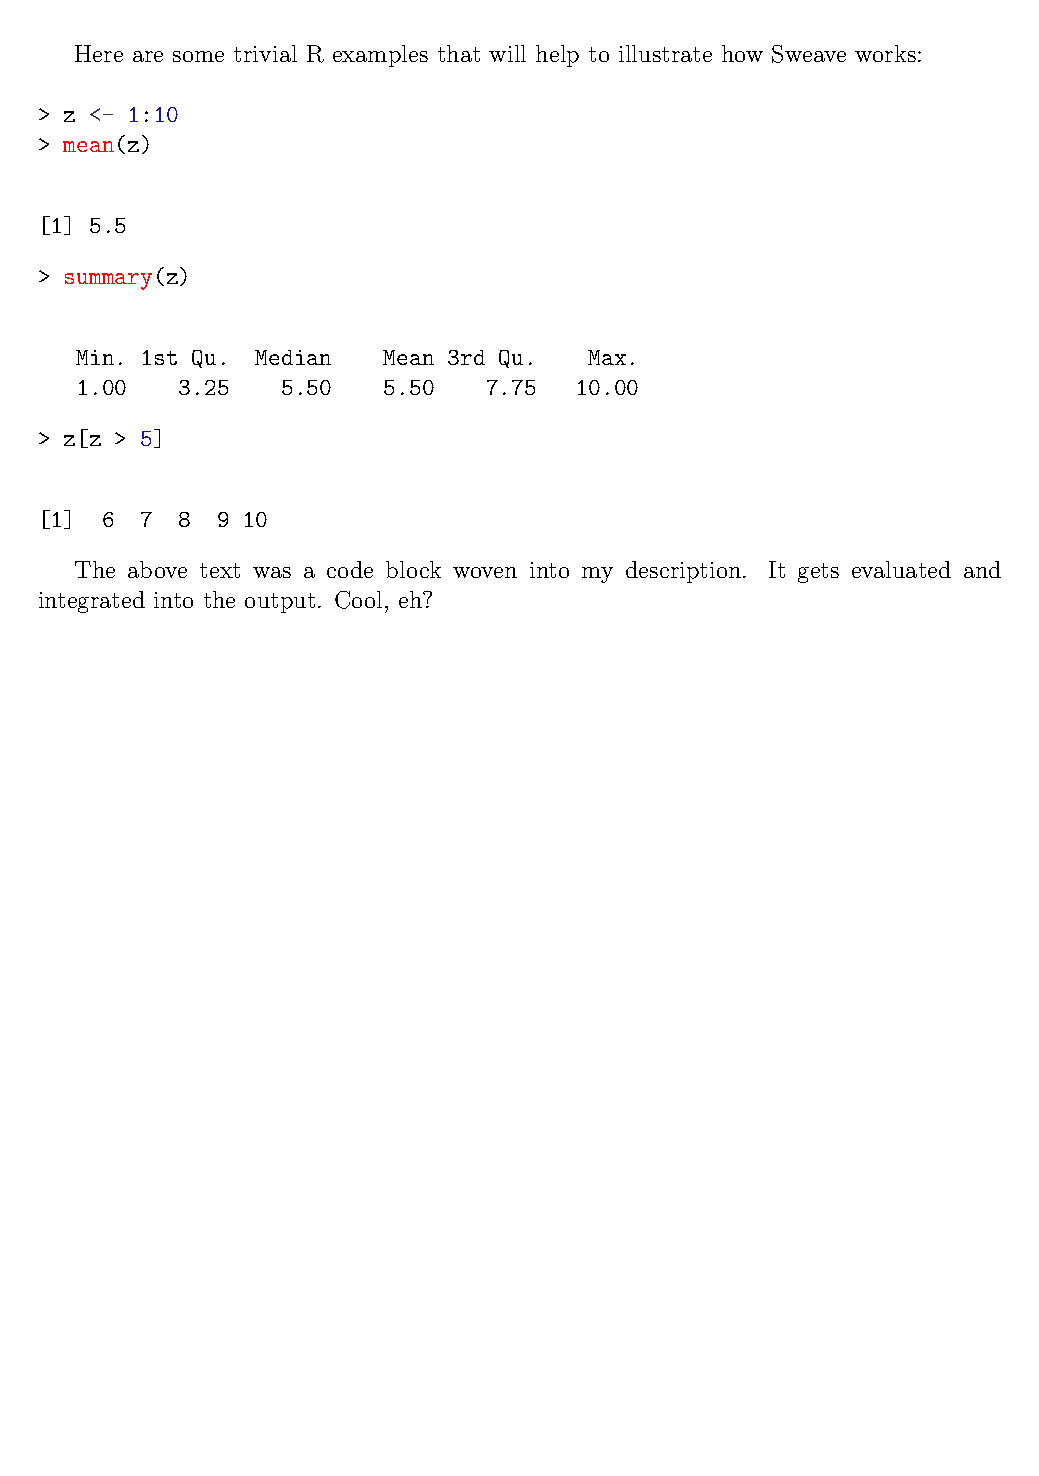
\includegraphics[width=\textwidth,trim=0in 5in 0in 0in,clip=true]{sweave-ex1.pdf}
\end{minipage}}
\end{center}


\end{frame}
%===========================================================


%===========================================================
\begin{frame}
  \frametitle{Fancier pgfSweave output}

There's a new package called pgfSweave that produce even nicer output (code highlighting, better figure formatting):

\begin{center}
\fcolorbox{black}{bg}{%
\begin{minipage}{.75\textwidth}
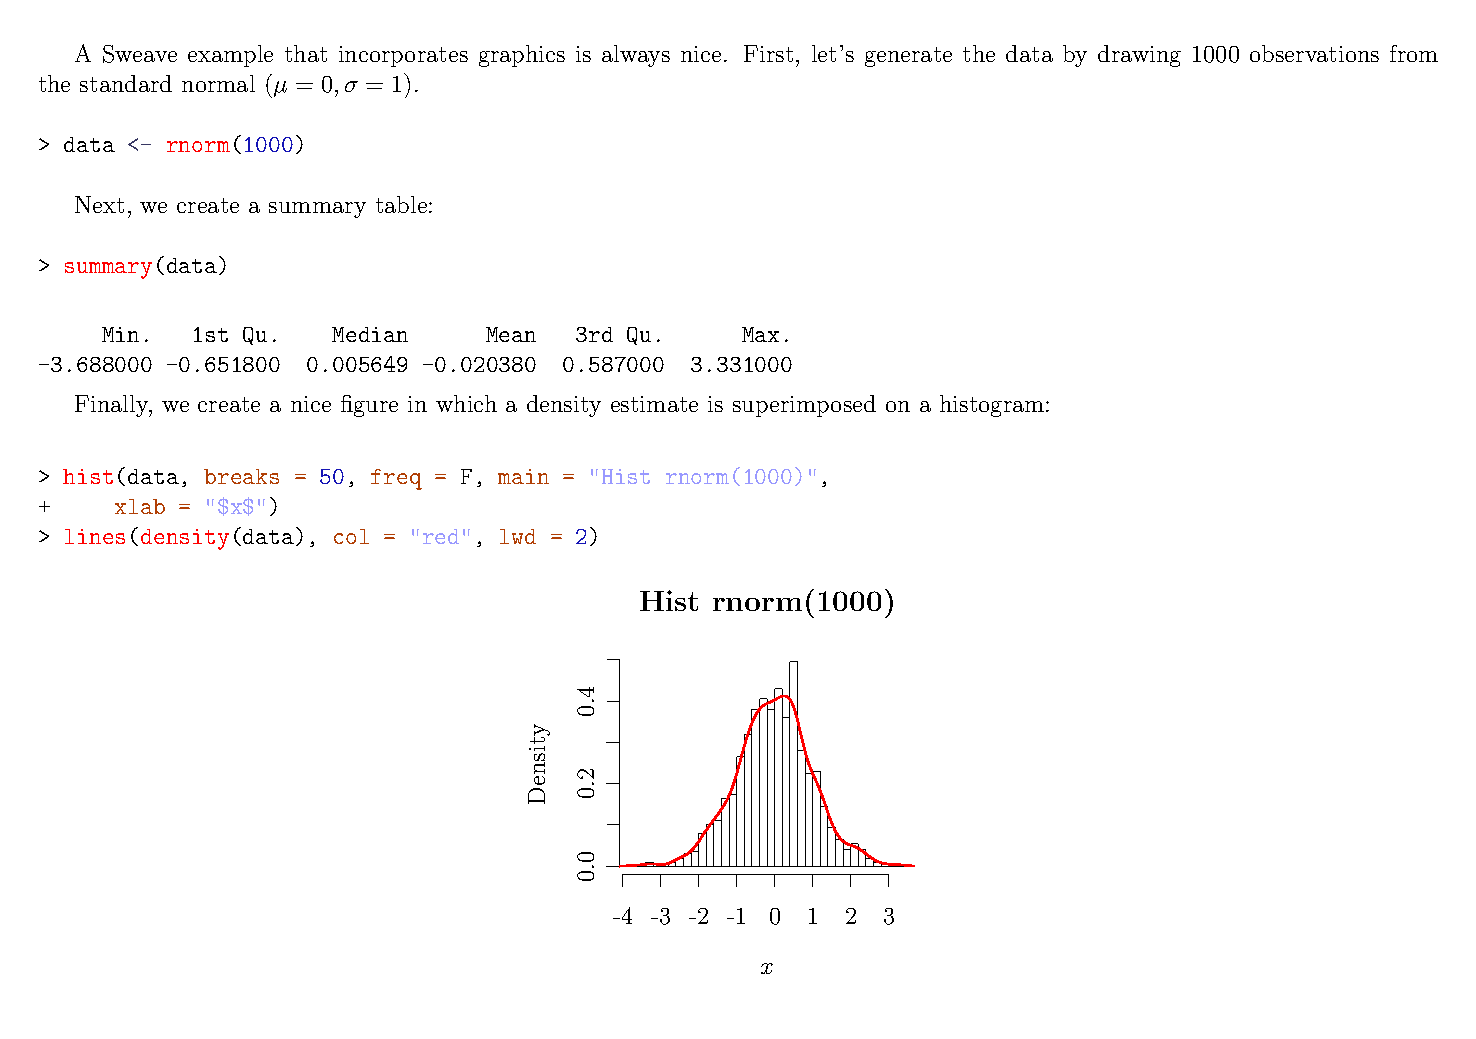
\includegraphics[width=\textwidth]{sweave-ex2.pdf}
\end{minipage}}
\end{center}


\end{frame}
%===========================================================



%===========================================================
\begin{frame}
  \frametitle{Things to Remember}

\begin{itemize}

 \item Try it out - programming involves experimentation
 \item Don't reinvent the wheel - it's usually worth spending some time finding out if someone has already written code that does what you need.
 \item Practice - learning to program, like learning a foreign language, requires lots of practice.
 \item Persist - many new tools/concepts can be hard to grasp at first. Keep plugging away until you get that `Aha!' moment
\end{itemize}


\end{frame}
%===========================================================


%===========================================================
\begin{frame}
  \frametitle{You might be surprised to find that...}

\begin{itemize}

 \item Programming is fun! (at least sometimes)
 \item Math is fun! (at least sometimes)
 \item Statistics is fun! (at least sometimes)
\bigskip
 \item Gaining new insights into how your biological system of interest works is fun! (always)

\end{itemize}

\end{frame}
%===========================================================



\end{document}
